\documentclass[border=12pt]{standalone}
\def\pgfsysdriver{pgfsys-dvisvgm.def}
\usepackage[dvisvgm]{xcolor}
\usepackage{xeCJK}
\setCJKmainfont{HaranoAjiGothic-Regular.otf}[BoldFont=HaranoAjiGothic-Bold.otf]
\setCJKsansfont{HaranoAjiGothic-Regular.otf}[BoldFont=HaranoAjiGothic-Bold.otf]
\usepackage{amsmath,amssymb,tikz,lmodern}
\usetikzlibrary{arrows.meta,positioning,calc,fit,backgrounds}
\renewcommand{\familydefault}{\sfdefault}
\definecolor{ink}{HTML}{25322F}
\definecolor{green}{HTML}{246657}
\definecolor{tint}{HTML}{EEF4F0}
\definecolor{soft}{HTML}{C6D2CC}
\definecolor{muted}{HTML}{52615B}
\newif\ifJapanese
\newcommand{\Tx}[2]{\ifJapanese #1\else #2\fi}
\newcommand{\Eff}{\overline{\operatorname{Eff}}}
\newcommand{\heading}[3]{{\color{green}\bfseries #1\quad\Tx{#2}{#3}}\\[5pt]}
% A white rectangle makes the complete citation label clickable, including spaces.
\newcommand{\refurl}[2]{\special{dvisvgm:raw <a xlink:href="#1" target="_blank" rel="noopener noreferrer">}{\setlength{\fboxsep}{0pt}\colorbox{white}{\color{green}\underline{\strut #2}}}\special{dvisvgm:raw </a>}}
\newcommand{\refedge}[3]{\refurl{\csname source#1\endcsname\string##page=#2}{#3}}
\newcommand{\SF}[2]{\refedge{sf}{#1}{#2}}
% GitHub's file preview does not support PDF page fragments.
\newcommand{\LA}[2]{\refurl{\sourcela}{#2}}
\newcommand{\Sch}[2]{\refedge{sch}{#1}{#2}}
\newcommand{\PS}[2]{\refedge{ps}{#1}{#2}}
\tikzset{
 card/.style={draw=soft,fill=white,rounded corners=2pt,align=left,text=ink,font=\fontsize{10.5}{14}\selectfont,inner xsep=12pt,inner ysep=10pt,text width=14.4cm},
 half/.style={card,text width=6.45cm,minimum height=2.05cm},
 result/.style={card,draw=green,fill=tint,line width=.9pt},
 reason/.style={align=left,text=muted,font=\fontsize{9}{12}\selectfont,inner sep=0pt,text width=12.7cm},
 branchreason/.style={reason,text width=5.95cm},
 edge/.style={-{Stealth[length=2.4mm]},draw=green,line width=1pt},
 wire/.style={draw=green,line width=1pt},
}
% Keep the arrow in a dedicated left gutter; explanations never cover it.
\newcommand{\flow}[3]{
 \coordinate (#2-from) at ($(#1.south)+(-6.9,0)$);
 \coordinate (#2-to) at ($(#2.north)+(-6.9,0)$);
 \draw[edge] (#2-from)--(#2-to);
 \node[reason,anchor=west] (#2-reason) at ($(#2-from)!.5!(#2-to)+(.55,0)$) {#3};
}


\newcommand{\CiteSource}[2]{\refurl{\csname source#1\endcsname}{#2}}

\expandafter\def\csname sourceU\endcsname{https://github.com/openai/math/blob/adc7f1241b42e322a6451854ab7e4b4c146bf78a/preprints/Uniform-Pluricanonical-Iitaka-Fibrations-October-3-2026/paper.pdf}
\expandafter\def\csname sourceLA\endcsname{https://github.com/openai/math/blob/adc7f1241b42e322a6451854ab7e4b4c146bf78a/preprints/Log-abundance-in-characteristic-zero-September-24-2026/paper.pdf}
\expandafter\def\csname sourceSD\endcsname{https://github.com/openai/math/blob/adc7f1241b42e322a6451854ab7e4b4c146bf78a/preprints/Arithmetic-Stein-degree-bounds-for-log-Calabi-Yau-pairs-September-25-2026/paper.pdf}
\expandafter\def\csname sourceUfour\endcsname{https://github.com/openai/math/blob/adc7f1241b42e322a6451854ab7e4b4c146bf78a/preprints/Uniform-effective-log-Iitaka-fibrations-for-fourfolds-September-26-2026/paper.pdf}
\expandafter\def\csname sourceR\endcsname{https://github.com/openai/math/blob/adc7f1241b42e322a6451854ab7e4b4c146bf78a/preprints/Relative-denominators-and-effective-systems-for-log-Calabi-Yau-fibrations-September-27-2026/paper.pdf}
\expandafter\def\csname sourceLog\endcsname{https://github.com/openai/math/blob/adc7f1241b42e322a6451854ab7e4b4c146bf78a/preprints/Uniform-log-Iitaka-fibrations-and-bounded-moduli-denominators-October-4-2026/uniform-log-iitaka.pdf}
\expandafter\def\csname sourceSLC\endcsname{https://github.com/openai/math/blob/adc7f1241b42e322a6451854ab7e4b4c146bf78a/preprints/Uniform-indices-for-semi-log-canonical-log-Calabi-Yau-pairs-October-5-2026/uniform-slc-index.pdf}
\expandafter\def\csname sourceBZ\endcsname{https://arxiv.org/pdf/1410.0938v2}

\Japanesefalse
\begin{document}
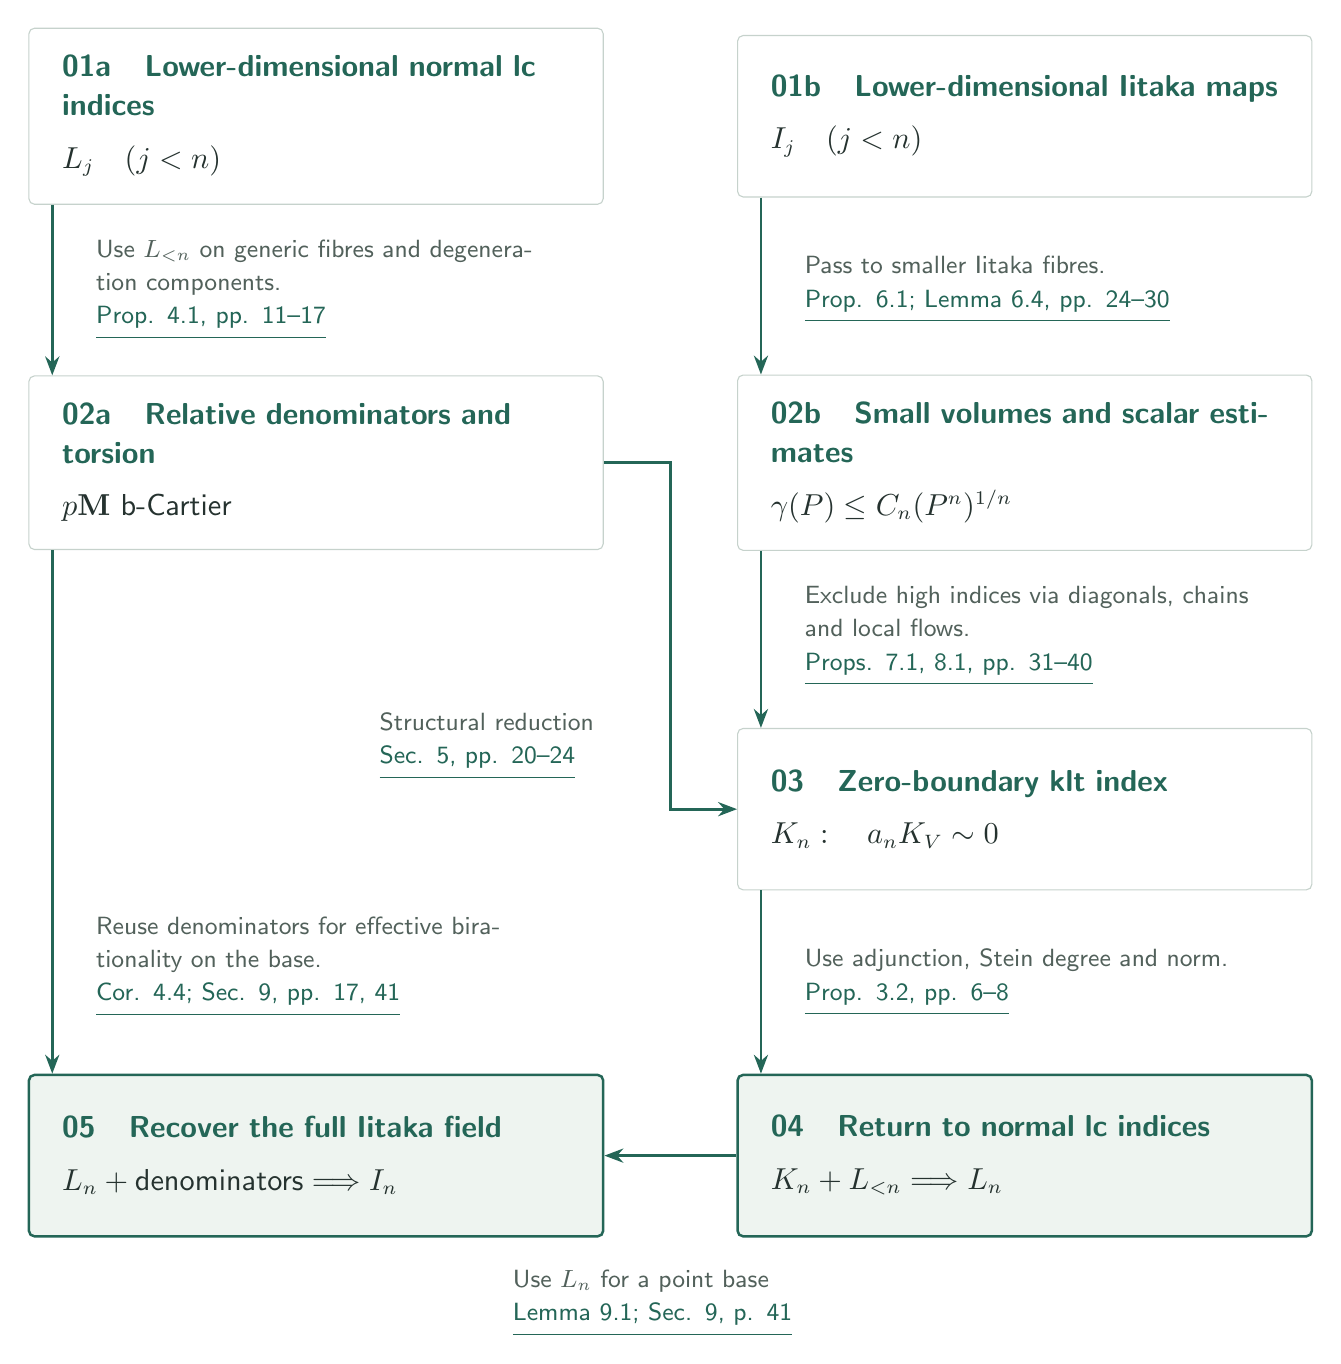
\begin{tikzpicture}
\node[half] (l) at (-4.5,0) {\heading{01a}{低次元の normal lc 指数}{Lower-dimensional normal lc indices}$L_j\quad(j<n)$};
\node[half] (i) at (4.5,0) {\heading{01b}{低次元の飯高写像}{Lower-dimensional Iitaka maps}$I_j\quad(j<n)$};
\node[half] (d) at (-4.5,-4.4) {\heading{02a}{相対的な分母と torsion}{Relative denominators and torsion}$p\mathbf M\ \text{b-Cartier}$};
\node[half] (s) at (4.5,-4.4) {\heading{02b}{小体積と scalar 評価}{Small volumes and scalar estimates}$\gamma(P)\le C_n(P^n)^{1/n}$};
\node[half] (k) at (4.5,-8.8) {\heading{03}{零境界 klt 指数}{Zero-boundary klt index}$K_n:\quad a_nK_V\sim0$};
\node[half,draw=green,fill=tint,line width=.9pt] (ln) at (4.5,-13.2) {\heading{04}{normal lc 指数へ戻す}{Return to normal lc indices}$K_n+L_{<n}\Longrightarrow L_n$};
\node[half,draw=green,fill=tint,line width=.9pt] (in) at (-4.5,-13.2) {\heading{05}{飯高体全体を回収する}{Recover the full Iitaka field}$L_n+\text{denominators}\Longrightarrow I_n$};
\draw[edge] ($(l.south)+(-3.35,0)$)--($(d.north)+(-3.35,0)$);
\node[branchreason,fill=white,anchor=west,text width=5.7cm] at (-7.3,-2.2) {\Tx{生成ファイバーと退化成分に $L_{<n}$ を使う。}{Use $L_{<n}$ on generic fibres and degeneration components.}\\\CiteSource{U}{Prop. 4.1, pp. 11--17}};
\draw[edge] ($(i.south)+(-3.35,0)$)--($(s.north)+(-3.35,0)$);
\node[branchreason,fill=white,anchor=west,text width=5.7cm] at (1.7,-2.2) {\Tx{小さい飯高ファイバーへ移る。}{Pass to smaller Iitaka fibres.}\\\CiteSource{U}{Prop. 6.1; Lemma 6.4, pp. 24--30}};
\draw[edge] ($(s.south)+(-3.35,0)$)--($(k.north)+(-3.35,0)$);
\node[branchreason,fill=white,anchor=west,text width=5.7cm] at (1.7,-6.6) {\Tx{対角積・鎖・局所 flow で高指数を排除する。}{Exclude high indices via diagonals, chains and local flows.}\\\CiteSource{U}{Props. 7.1, 8.1, pp. 31--40}};
\draw[edge] (d.east)--(0,-4.4)--(0,-8.8)--(k.west);
\node[branchreason,anchor=west,text width=3.0cm] at (-3.7,-8.0) {\Tx{構造帰着に使用}{Structural reduction}\\\CiteSource{U}{Sec. 5, pp. 20--24}};
\draw[edge] ($(k.south)+(-3.35,0)$)--($(ln.north)+(-3.35,0)$);
\node[branchreason,fill=white,anchor=west,text width=5.7cm] at (1.7,-11.0) {\Tx{adjunction と Stein 次数・norm を使う。}{Use adjunction, Stein degree and norm.}\\\CiteSource{U}{Prop. 3.2, pp. 6--8}};
\draw[edge] ($(d.south)+(-3.35,0)$)--($(in.north)+(-3.35,0)$);
\node[branchreason,fill=white,anchor=west,text width=5.5cm] at (-7.3,-10.8) {\Tx{分母を再利用し、底に有効双有理性を適用する。}{Reuse denominators for effective birationality on the base.}\\\CiteSource{U}{Cor. 4.4; Sec. 9, pp. 17, 41}};
\draw[edge] (ln.west)--(in.east);
\node[reason,text width=4cm,anchor=north] at (0,-14.65) {\Tx{底が点の場合には $L_n$}{Use $L_n$ for a point base}\\\CiteSource{U}{Lemma 9.1; Sec. 9, p. 41}};
\end{tikzpicture}
\end{document}
